\documentclass[a4paper,colorlinks=true,linkcolor=blue,urlcolor=blue,citecolor=green,bookmarks=true]{article}

% 基础宏包
\usepackage{ctex}              % 中文支持
\usepackage{graphicx}          % 图片支持
\usepackage{amsmath}           % 数学公式
\usepackage{amssymb}          % 数学符号
\usepackage{geometry}          % 页面设置
\usepackage{fancyhdr}          % 页眉页脚
\usepackage{lastpage}          % 获取总页数
\usepackage{zhnumber}          % 中文数字
\usepackage{float}             % 浮动体设置
\usepackage{subcaption}        % 支持子图

% 页面设置
\geometry{a4paper,top=2.5cm,bottom=2.5cm,left=2.5cm,right=2.5cm}

% 浮动体设置
\renewcommand{\textfraction}{0.05}
\renewcommand{\topfraction}{0.95}
\renewcommand{\bottomfraction}{0.95}
\renewcommand{\floatpagefraction}{0.35}
\setcounter{topnumber}{5}
\setcounter{bottomnumber}{5}
\setcounter{totalnumber}{10}

% 引入样式文件
% 基础包引用
\usepackage{amsmath}
\usepackage{graphicx}
\usepackage{float}
\usepackage{setspace}
\usepackage{xargs}
\usepackage{nameref}
\usepackage{appendix}
\usepackage{cite}
\usepackage{hyperref}
\usepackage{fancyref}
\usepackage{scrextend}

% 颜色定义
\usepackage[dvipsnames]{xcolor}
\definecolor{cleanOrange}{HTML}{D14D00}
\definecolor{cleanYellow}{HTML}{FFFF99}
\definecolor{cleanBlue}{HTML}{3d0099}

% 通用命令
\newcommand\tab[1][1cm]{\hspace*{#1}}
\hypersetup{colorlinks=true, linkcolor=black}
\interfootnotelinepenalty=10000

% 注释和标记
\usepackage[colorinlistoftodos,prependcaption,textsize=footnotesize]{todonotes}
\newcommandx{\commred}[2][1=]{\textcolor{Red}{\todo[linecolor=red,backgroundcolor=red!25,bordercolor=red,#1]{#2}}}
\newcommandx{\commblue}[2][1=]{\textcolor{Blue}{\todo[linecolor=blue,backgroundcolor=blue!25,bordercolor=blue,#1]{#2}}}
\newcommandx{\commgreen}[2][1=]{\textcolor{OliveGreen}{\todo[linecolor=OliveGreen,backgroundcolor=OliveGreen!25,bordercolor=OliveGreen,#1]{#2}}}
\newcommandx{\commpurp}[2][1=]{\textcolor{Plum}{\todo[linecolor=Plum,backgroundcolor=Plum!25,bordercolor=Plum,#1]{#2}}}

% 代码和注释
\def\code#1{{\tt #1}}
\def\note#1{\noindent{\bf [Note: #1]}}

% 附录格式
\makeatletter
\def\@seccntformat#1{\@ifundefined{#1@cntformat}%
   {\csname the#1\endcsname\quad}%
   {\csname #1@cntformat\endcsname}%
}
\let\oldappendix\appendix
\renewcommand\appendix{%
    \oldappendix
    \newcommand{\section@cntformat}{\appendixname~\thesection\quad}
}
\makeatother 
% 页面布局设置
\usepackage{geometry}
\geometry{a4paper,left=2.3cm,right=2.3cm,top=2.7cm,bottom=2.7cm}

% 页眉页脚
\usepackage{fancyhdr}
\usepackage{lastpage}
\pagestyle{fancy}
\renewcommand{\headrulewidth}{0.1pt}
\renewcommand{\footrulewidth}{0pt}

% 章节格式
\usepackage{sectsty}
\sectionfont{\LARGE}
\subsectionfont{\Large}
\subsubsectionfont{\large}

% 表格设置
\usepackage{tabularx}
\usepackage{booktabs}
\usepackage{multirow}

% 图表设置
\usepackage{caption}
\usepackage{subfigure}
\setlength{\textfloatsep}{10mm}

% 标题线设置
\providecommand{\HRule}{\rule{\linewidth}{0.5mm}}
\providecommand{\HRulegrossa}{\rule{\linewidth}{1.2mm}} 
% 字体和编码设置
\usepackage{ctex}
\usepackage[utf8]{inputenc}
\usepackage[british,UKenglish]{babel}

% 字体命令
\newcommand{\cleancode}[1]{\begin{addmargin}[3em]{3em}\texttt{\textcolor{cleanOrange}{#1}}\end{addmargin}}
\newcommand{\cleanstyle}[1]{\text{\textcolor{cleanOrange}{\texttt{#1}}}} 
% 代码样式设置
\usepackage[T1]{fontenc}
\usepackage[scaled=0.82]{beramono}
\usepackage{microtype}
\usepackage[procnames]{listings}

% 代码颜色定义
\definecolor{dkgreen}{rgb}{0,0.6,0}
\definecolor{gray}{rgb}{0.5,0.5,0.5}
\definecolor{mauve}{rgb}{0.58,0,0.82}

% 基础代码样式
\lstset{
  frame=tb,
  aboveskip=3mm,
  belowskip=3mm,
  showstringspaces=false,
  columns=fixed,
  basicstyle={\small\ttfamily},
  numbers=left,
  numberstyle=\tiny\color{gray},
  keywordstyle=\color{blue},
  commentstyle=\color{dkgreen},
  stringstyle=\color{mauve},
  frame=single,
  breaklines=true,
  breakatwhitespace=true,
  tabsize=2
}

% Scala语言定义
\lstdefinelanguage{scala}{
  morekeywords={abstract,case,catch,class,def,
    do,else,extends,false,final,finally,
    for,if,implicit,import,match,mixin,
    new,null,object,override,package,
    private,protected,requires,return,sealed,
    super,this,throw,trait,true,try,
    type,val,var,while,with,yield},
  sensitive=true,
  morecomment=[l]{//},
  morecomment=[n]{/*}{*/},
  morestring=[b]",
  morestring=[b]',
  morestring=[b]"""
}

% 语言环境定义
\lstnewenvironment{scala}[1][]
{\lstset{language=scala,#1}}
{}
\lstnewenvironment{cpp}[1][]
{\lstset{language=C++,#1}}
{}
\lstnewenvironment{bash}[1][]
{\lstset{language=bash,#1}}
{}
\lstnewenvironment{verilog}[1][]
{\lstset{language=verilog,#1}}
{} 

% 图片路径
\graphicspath{{fig/}}

% 使用natbib和plainurl风格
\usepackage[numbers,sort&compress,square,comma]{natbib}
\bibliographystyle{unsrtnat}

% 参考文献处理增强
\usepackage{hyperref}
\usepackage{url}
\usepackage{xurl}
\renewcommand{\UrlFont}{\ttfamily\color{blue}\small}

% 确保文献内含中文字符时正确编译
\usepackage{etoolbox}
\patchcmd{\thebibliography}{\sloppy}{\sloppy\raggedright}{}{}

% 自定义参考文献样式
\makeatletter
\renewcommand\@biblabel[1]{{\bf [#1]}}
\def\@cite#1#2{[{#1\if@tempswa , #2\fi}]}
\renewcommand{\bibfont}{\small}
\setlength{\bibsep}{1.2ex}
\makeatother

% 美化URL显示
\usepackage{xurl}
\renewcommand{\UrlFont}{\ttfamily\color{blue}\small}

% 伪代码设置
\usepackage{algorithm}  
\usepackage{algorithmicx}  
\usepackage{algpseudocode}  
\floatname{algorithm}{Algorithm}  
\renewcommand{\algorithmicrequire}{\textbf{Input:}}  
\renewcommand{\algorithmicensure}{\textbf{Output:}} 
\usepackage{lipsum}  

% 定义中英文摘要环境
\makeatletter
% 中文摘要环境
\newenvironment{cnabstract}{
    \par\small
    \noindent\mbox{}\par\vspace{-\baselineskip}
    \par\songti\parindent 2em
    }
    {\par\vspace{1em}}

% 英文摘要环境
\newenvironment{enabstract}{
    \par\small
    \noindent\mbox{}\par\vspace{-\baselineskip}
    \par\parindent 2em
    }
    {\par\vspace{1em}}
\makeatother

\makeatletter
\providecommand{\breakablealgorithm}{%
  \begin{center}
     \refstepcounter{algorithm}%
     \hrule height.8pt depth0pt \kern2pt%
     \renewcommand{\caption}[2][\relax]{%
      {\raggedright\textbf{\ALG@name~\thealgorithm} ##2\par}%
      \ifx\relax##1\relax
         \addcontentsline{loa}{algorithm}{\protect\numberline{\thealgorithm}##2}%
      \else
         \addcontentsline{loa}{algorithm}{\protect\numberline{\thealgorithm}##1}%
      \fi
      \kern2pt\hrule\kern2pt
     }
  \end{center}
}
\makeatother

%-------------------------页眉页脚--------------
\pagestyle{fancy}
\lhead{\kaishu \leftmark}
\rhead{\kaishu 并行程序设计实验报告}
\lfoot{}
\cfoot{\thepage}
\rfoot{}

%--------------------文档内容--------------------

\begin{document}
\renewcommand{\contentsname}{目录}
\renewcommand{\appendixname}{附录}
\renewcommand{\appendixpagename}{附录}
\renewcommand{\refname}{参考文献} 
\renewcommand{\figurename}{图}
\renewcommand{\tablename}{表}
\renewcommand{\abstractname}{摘要}
\renewcommand{\today}{\number\year 年 \number\month 月 \number\day 日}

\renewcommand {\thefigure}{\thesection{}.\arabic{figure}}%图片按章标号
\renewcommand{\figurename}{图}
\renewcommand{\contentsname}{目录}  
\cfoot{\thepage\ of \pageref{LastPage}}%当前页 of 总页数

% 封面
\begin{titlepage}
    \begin{center}
    
\includegraphics[width=0.6\textwidth]{NKU.png}\\[1cm]
    \vspace{20mm}
		\textbf{\huge\textbf{\kaishu{计算机学院}}}\\[0.5cm]
		\textbf{\huge{\kaishu{并行程序设计报告}}}\\[2.3cm]
		\textbf{\Huge\textbf{\kaishu{NTT SIMD优化实验报告}}}

		\vspace{\fill}
    
    \centering
    \textsc{\LARGE \kaishu{姓名\ :\ 张三}}\\[0.5cm]
    
    \vfill
    {\Large \today}
    \end{center}
\end{titlepage}

% 中文摘要
\clearpage
\phantomsection
\begin{center}{\zihao{4}\songti\bfseries{摘\quad 要}}\end{center}\par\vspace{0.5em}
\addcontentsline{toc}{section}{摘要}
\begin{cnabstract}
本报告探讨了数论变换(NTT)的SIMD优化实现,重点研究不同优化策略在x86-64(AVX2)和ARM(NEON)平台上的性能表现。我们实现了朴素NTT、DIF结构优化、SIMD向量化以及DIF+SIMD联合优化四种方案,并在不同模数(469762049、1337006139375617和7696582450348003)下进行了性能对比。实验结果表明:1)在AVX2平台(256位宽向量寄存器)上,DIF+AVX2联合优化在标准模数下提供了约35\%的加速;2)在NEON平台(128位宽向量寄存器)上,DIF结构优化表现最佳,提供了约4倍加速,而DIF+NEON联合优化反而性能下降;3)对于超大模数,我们探索了基于中国剩余定理的拼接技术,成功实现了SIMD优化。本研究揭示了硬件特性与算法结构的匹配关系对优化效果的关键影响,为多项式乘法在密码学等领域的高效实现提供了重要参考。附录中提供了NEON平台的实验结果截图。代码仓库可访问:\href{https://github.com/aokimi0/parallel-programming}{GitHub}。

\vspace{1em}
\noindent\textbf{关键词:}数论变换;SIMD优化;向量化计算;多项式乘法;蝴蝶变换
\end{cnabstract}

% 英文摘要
\phantomsection
\begin{center}{\zihao{4}\bfseries{Abstract}}\end{center}\par\vspace{0.5em}
\addcontentsline{toc}{section}{Abstract}
\begin{enabstract}
This report investigates SIMD optimization strategies for Number Theoretic Transform (NTT), focusing on performance across x86-64 (AVX2) and ARM (NEON) platforms. We implemented four versions: naive NTT, DIF-structured optimization, SIMD vectorization, and combined DIF+SIMD optimization, testing them with different moduli (469762049, 1337006139375617, and 7696582450348003). Results show that: 1) On the AVX2 platform (256-bit vector registers), DIF+AVX2 joint optimization achieved approximately 35\% speedup for standard moduli; 2) On the NEON platform (128-bit vector registers), DIF structural optimization provided the best performance with a 4-fold acceleration, while surprisingly, the DIF+NEON joint optimization performed worse than DIF alone; 3) For large moduli, we explored a Chinese Remainder Theorem-based technique that successfully implemented SIMD optimization. This study reveals the critical impact of matching hardware characteristics with algorithm structure, providing important references for efficient polynomial multiplication implementation in cryptography and other fields. Experimental result screenshots for the NEON platform are provided in the appendix. Full code is available at: \href{https://github.com/aokimi0/parallel-programming}{GitHub}.

\vspace{1em}
\noindent\textbf{Keywords:} Number Theoretic Transform; SIMD Optimization; Vectorized Computing; Polynomial Multiplication; Butterfly Operation
\end{enabstract}

% 目录
\clearpage
\tableofcontents
\clearpage

\section{一级标题}


\subsection{二级标题}
NTT(Number Theoretic Transform)是将FFT的复数单位根替换为有限域上的单位根,所有运算均在模$p$的有限域$Z_p$上进行。对于质数$p$,我们定义$Z_p=\{0,1,2,...,p-1\}$,其中元素的加减乘运算均在模$p$下进行\cite{harvey2014}。

NTT的关键是选择适当的模数$p$和原根$g$,使得$n|(p-1)$,其中$n$是变换长度(通常为2的幂次)。在本实验中,我们使用的模数均满足$p = a \times 4^k + 1$的形式,且原根均为3\cite{longa2016}。

\begin{lstlisting}[language=C++]
class M {
public:
    static u32 m, g, i, r;
    static int l, w;
    static void sm(u32 mm, u32 gg) {
        m = mm;
        g = gg;
        w = 8 * sizeof(u32);
        i = mi(m);
        r = -u64(m) % m;
        l = __builtin_ctzll(m - 1);
    }
    static u32 mi(u32 n, int e = 6, u32 x = 1) {
        return e == 0 ? x : mi(n, e - 1, x * (2 - x * n));
    }
    M() : x(0) {}
    M(u32 n) : x(init(n)) {}
    static u32 modulus() { return m; }
    static u32 init(u32 w_) { return reduce(u64(w_) * r); }
    static u32 reduce(const u64 w_) {
        return u32(w_ >> w) + m - u32((u64(u32(w_) * i) * m) >> w);
    }
    static M om() {
        return M(g).qp((m - 1) >> l);
    }
    M &operator+=(const M &o) {
        x += o.x;
        return *this;
    }
    M &operator-=(const M &o) {
        x += 3 * m - o.x;
        return *this;
    }
    M &operator*=(const M &o) {
        x = reduce(u64(x) * o.x);
        return *this;
    }
    M operator+(const M &o) const { return M(*this) += o; }
    M operator-(const M &o) const { return M(*this) -= o; }
    M operator*(const M &o) const { return M(*this) *= o; }
    u32 v() const { return reduce(x) % m; }
    void set(u32 n) { x = n; }
    M qp(u32 e) const {
        M ret = M(1);
        for (M base = *this; e; e >>= 1, base *= base)
            if (e & 1) ret *= base;
        return ret;
    }
    M iv() const { return qp(m - 2); }
    alignas(4) u32 x;
};
\end{lstlisting}

此类实现了Montgomery规约下的模运算,包括加、减、乘、幂等操作。\verb|reduce|函数是Montgomery乘法的核心,避免了传统的模运算中昂贵的除法操作。


\subsubsection{x86-64平台}
\begin{itemize}
  \item \textbf{处理器}:12th Gen Intel(R) Core(TM) i5-12500H(2.5-4.5GHz)
  \item \textbf{核心数}:16(8P+8E)
  \item \textbf{内存}:7.6GiB
  \item \textbf{系统}:WSL2 Ubuntu 24.04,内核 5.15.167.4
  \item \textbf{指令集}:SSE、AVX2等
  \item \textbf{向量寄存器}:256位宽(AVX2),每次可处理8个32位整数
  \item \textbf{编译器}:GCC 13.3.0
  \item \textbf{编译命令}:\verb|g++ -O2 -mavx2 -std=c++17|
  \item \textbf{数据集}:n = 1000、10000、100000,模数p = 469762049、1337006139375617、7696582450348003
\end{itemize}


\begin{table}[H]
\centering
\caption{AVX2平台不同实现性能对比}
\resizebox{\textwidth}{!}{%
\begin{tabular}{|c|C{5cm}|C{5cm}|C{5cm}|}
\hline
\textbf{实现/模数} & \textbf{469762049} & \textbf{1337006139375617*} & \textbf{7696582450348003**} \\
\hline
朴素NTT & 0.021304 / 0.090902 / 0.279013 & 0.033612 / 0.053125 / 0.411691 & 0.034052 / 0.101207 / 0.615350 \\
\hline
DIF优化 & 0.019207 / 0.068735 / 0.243873 & 0.040841 / 0.059597 / 0.360514 & 0.031898 / 0.085399 / 0.493560 \\
\hline
AVX2优化 & 0.018449 / 0.075861 / 0.229530 & 0.031264 / 0.106777 / 0.374022 & 0.032373 / 0.089031 / 0.384058 \\
\hline
DIF+AVX2优化 & 0.016924 / 0.042322 / 0.183502 & 0.033325 / 0.051157 / 0.448294 & 0.028505 / 0.066871 / 0.278603 \\
\hline
\end{tabular}%
}
\vspace{0.3em}
\begin{flushleft}
\normalsize{单位:秒(s),每个单元格内三个数据分别对应n=1000、n=10000、n=100000}\\
\normalsize{* 对于超大模数1337006139375617,由于超出32位整数范围且不能分解为NTT友好的小模数,所有带SIMD标记的实现实际上使用的是朴素NTT算法。各实现之间表现出的性能差异主要来自系统负载、缓存状态等随机波动因素,而非算法结构或SIMD优化的差异。}\\
\normalsize{** 对于7696582450348003模数,通过小模数+CRT拼接技术实现SIMD优化,即将其分解为两个NTT友好的小模数7340033和104857601,分别进行SIMD加速计算,再通过中国剩余定理合并结果}
\end{flushleft}
\end{table}


\begin{figure}[H]
  \centering
  \begin{subfigure}[b]{0.32\textwidth}
    \centering
    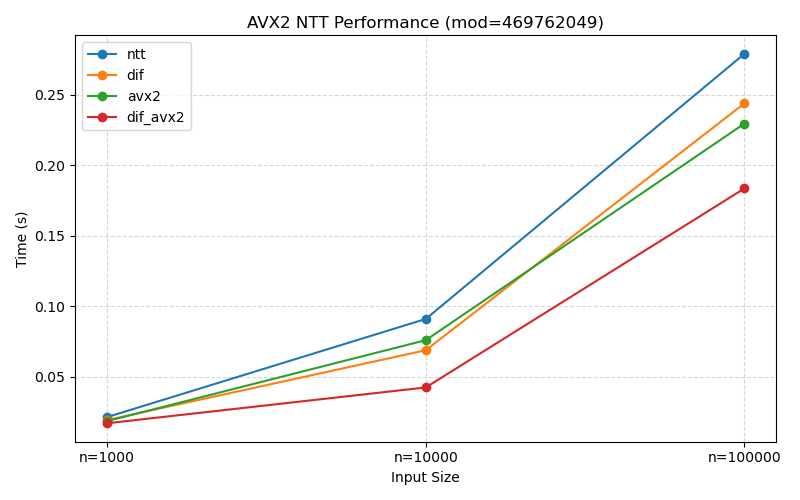
\includegraphics[width=\textwidth]{avx2_469762049.png}
    \caption{AVX2性能对比 (mod=469762049)}
    \label{fig:avx2_469762049}
  \end{subfigure}
  \hfill
  \begin{subfigure}[b]{0.32\textwidth}
    \centering
    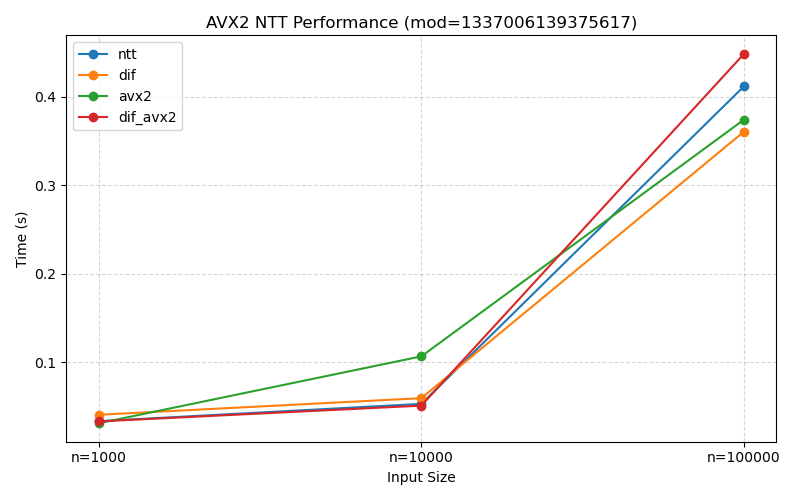
\includegraphics[width=\textwidth]{avx2_1337006139375617.png}
    \caption{AVX2性能对比 (mod=1337006139375617)}
    \label{fig:avx2_1337006139375617}
  \end{subfigure}
  \hfill
  \begin{subfigure}[b]{0.32\textwidth}
    \centering
    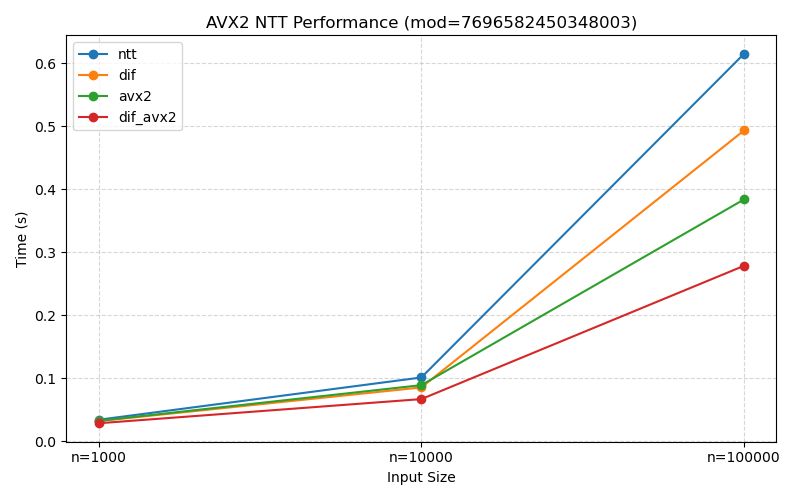
\includegraphics[width=\textwidth]{avx2_7696582450348003.png}
    \caption{AVX2性能对比 (mod=7696582450348003)}
    \label{fig:avx2_7696582450348003}
  \end{subfigure}
  \caption{AVX2平台不同模数下的性能对比}
  \label{fig:avx2_performance}
\end{figure}

\begin{figure}[H]
  \centering
  \begin{subfigure}[b]{0.32\textwidth}
    \centering
    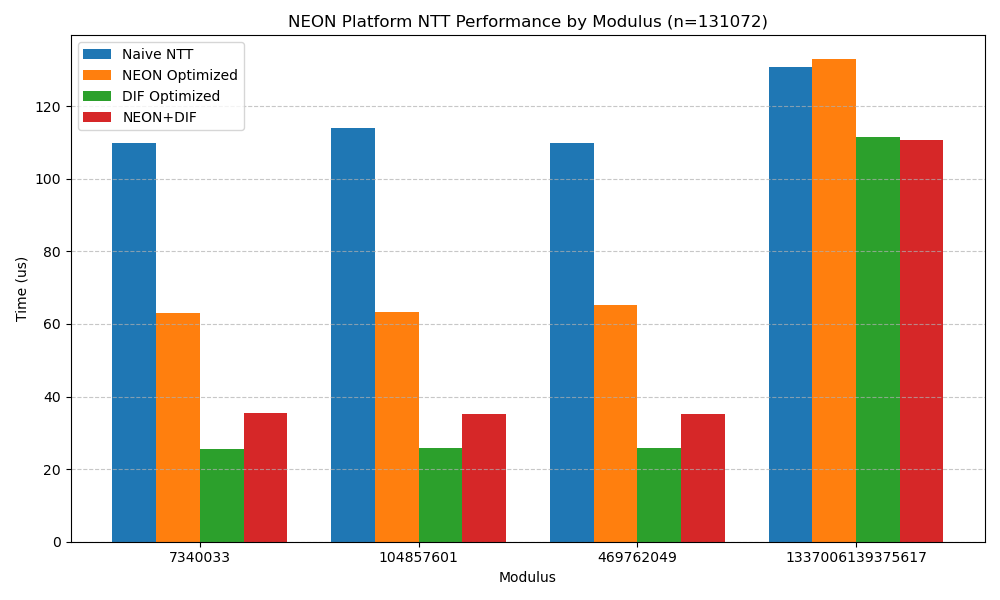
\includegraphics[width=\textwidth]{neon_modulus_comparison.png}
    \caption{NEON平台不同模数对比}
    \label{fig:neon_modulus}
  \end{subfigure}
  \hfill
  \begin{subfigure}[b]{0.32\textwidth}
    \centering
    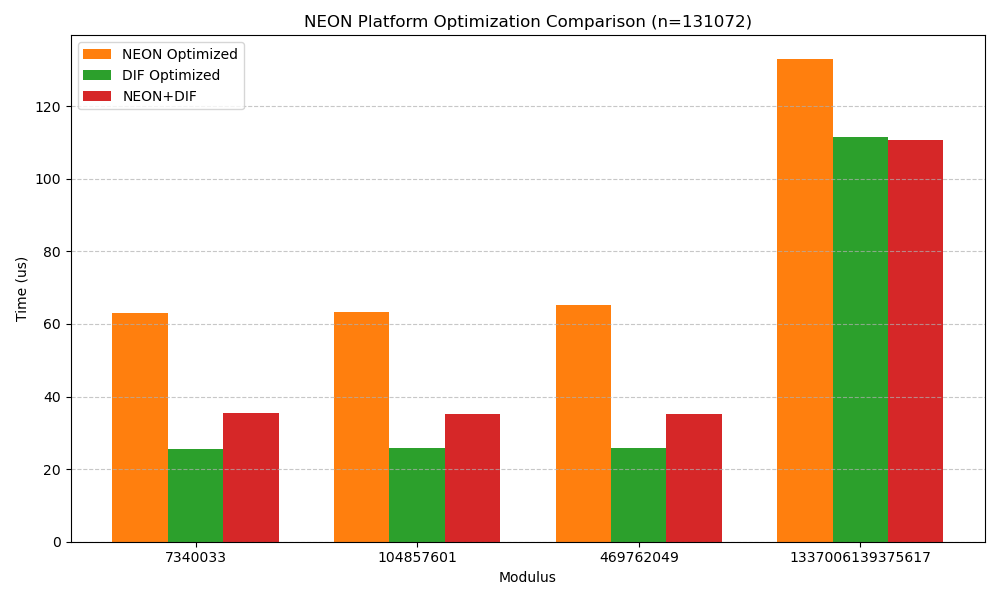
\includegraphics[width=\textwidth]{neon_optimization_comparison.png}
    \caption{NEON平台优化方法对比}
    \label{fig:neon_optimization}
  \end{subfigure}
  \hfill
  \begin{subfigure}[b]{0.32\textwidth}
    \centering
    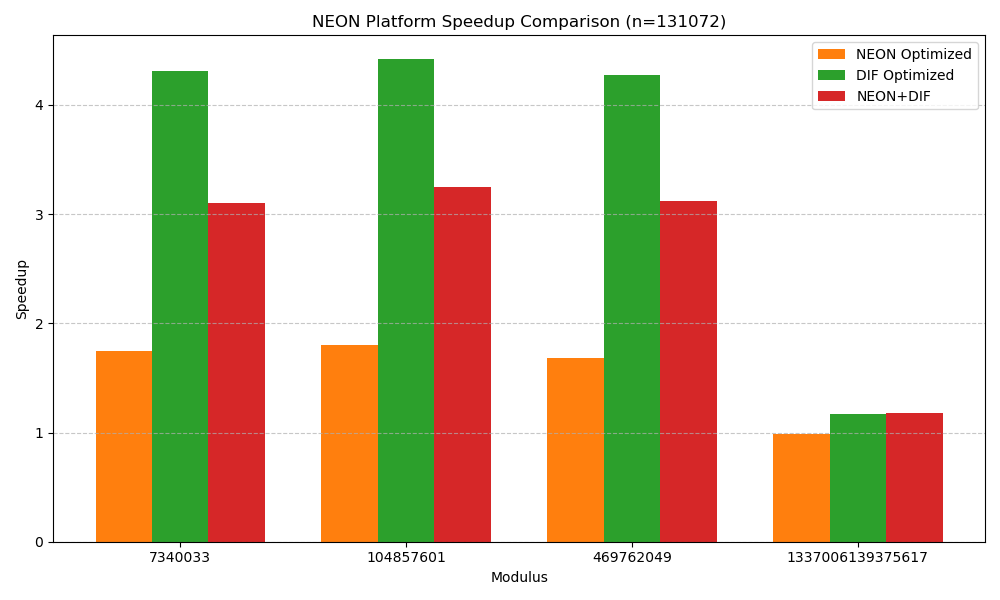
\includegraphics[width=\textwidth]{neon_speedup_comparison.png}
    \caption{NEON平台加速比对比}
    \label{fig:neon_speedup}
  \end{subfigure}
  \caption{NEON平台性能分析图表}
  \label{fig:neon_performance}
\end{figure}

\clearpage
\phantomsection
\addcontentsline{toc}{section}{参考文献}
% 使用natbib配合biblatex的方式处理参考文献
\renewcommand{\bibname}{参考文献}
\nocite{*} % 显示全部参考文献,即使未被引用
\bibliography{reference}

\clearpage
\phantomsection
\appendix
\addcontentsline{toc}{section}{附录}
\section*{附录A:NEON平台实验结果截图}
\renewcommand{\thesubsection}{A.\arabic{subsection}}

% 重置图表计数器并修改图表编号格式
\setcounter{figure}{0}
\renewcommand{\thefigure}{A.\arabic{figure}}

\subsection{朴素NTT实现}
\begin{figure}[H]
  \centering
  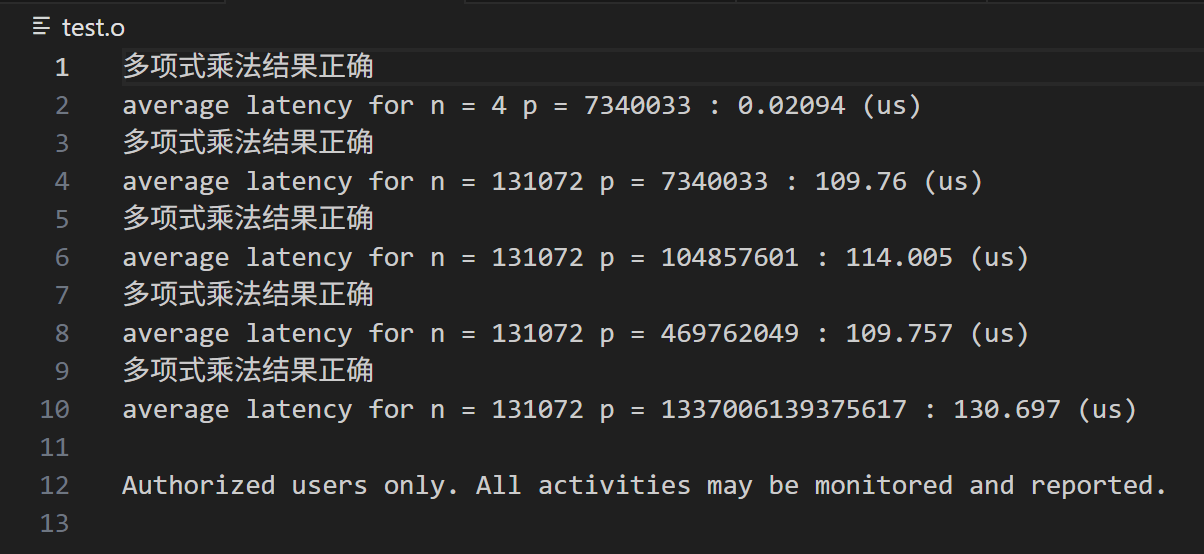
\includegraphics[width=0.7\textwidth]{ntt.png}
  \caption{朴素NTT实现性能}
  \label{fig:ntt_screenshot}
\end{figure}


\end{document} 